% Figure — Système asservi en réaction négative (EANA3, chapitre 1).
% D'après les notes externes [tableau-2020-c01, p. 2] et [notes-2023-c01, p. 1], redessinée.
% Rendu SVG :
%   latex -output-directory=<dossier temporaire> 01-schema-bloc-contre-reaction.tex
%   dvisvgm --no-fonts --exact-bbox -o 01-schema-bloc-contre-reaction.svg <dossier temporaire>/01-schema-bloc-contre-reaction.dvi
\documentclass[tikz,border=4pt]{standalone}
\usepackage[T1]{fontenc}
\usepackage[utf8]{inputenc}
\usepackage{sansmath}
\renewcommand{\familydefault}{\sfdefault}
\usetikzlibrary{positioning,arrows.meta,calc,shapes.geometric}
\begin{document}
\sansmath
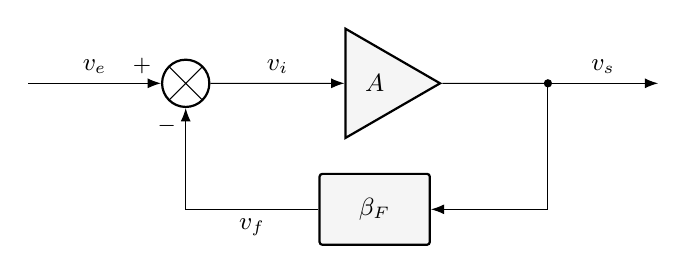
\begin{tikzpicture}[>=Latex, font=\small,
    bloc/.style={draw, thick, rounded corners=1pt, minimum height=9mm, minimum width=14mm, align=center, fill=black!4},
    ampli/.style={draw, thick, isosceles triangle, isosceles triangle apex angle=60, minimum height=12mm, fill=black!4, inner sep=1pt}]
  \coordinate (e) at (0,0);
  \node[draw, circle, thick, inner sep=0pt, minimum size=6mm] (som) at (2,0) {};
  \draw ($(som.center)+(45:3mm)$) -- ($(som.center)+(225:3mm)$) ($(som.center)+(135:3mm)$) -- ($(som.center)+(-45:3mm)$);
  \node[ampli] (A) at (4.4,0) {$A$};
  \coordinate (n) at (6.6,0);
  \coordinate (s) at (8,0);
  \node[bloc] (b) at (4.4,-1.6) {$\beta_F$};
  \draw[->] (e) -- node[above] {$v_e$} (som.west);
  \node[above left=0mm and 0mm of som.west, font=\footnotesize] {$+$};
  \draw[->] (som.east) -- node[above] {$v_i$} (A.west);
  \draw (A.east) -- (n);
  \draw[->] (n) -- node[above] {$v_s$} (s);
  \fill (n) circle (1.5pt);
  \draw[->] (n) |- (b.east);
  \draw[->] (b.west) -| node[pos=0.25, below] {$v_f$} (som.south);
  \node[below left=0mm and 0mm of som.south, font=\footnotesize] {$-$};
\end{tikzpicture}
\end{document}
